\chapter{机械能定理}

\section*{A 组}
\vspace{0.3cm}
\textbf{3-1} 图中的 $A_{3}BCD_{3}$ 是一条长轨道, 其中 $A_{3}B$ 是斜面段, $CD_{3}$ 是水平段, BC 是与 $A_{3}B$ 和 $CD_{3}$ 都相切的一小段圆弧. 一个小球与斜面段各处摩擦因数相同, 小球与水平段各处摩擦因数也都相同，但这两个摩擦因数未必相同。小球依次由 $A_{1}, A_{2}, A_{3}$ 从静止开始滑下，最后分别停留在 $D_{1}, D_{2}, D_{3}$ 点。已知 $h_{2} - h_{1} = 0.30 \mathrm{~m}, h_{3} - h_{2} = 0.48 \mathrm{~m}, \overline{D_{1} D_{2}} = 1.5 \mathrm{~m}$ ，试求 $\overline{D_{2} D_{3}}$ 长度。

\begin{center}
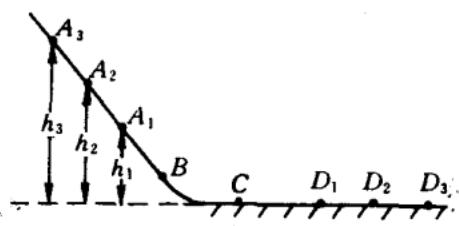
\includegraphics[width=0.3\textwidth]{figures/图3_1.jpg}
\end{center}

\vfill

\textbf{3-2} 某人心脏每搏动一次泵出 80.0 mL 的血液, 一次搏动过程中心脏主动脉平均压强为 120 mmHg. 已知此人脉搏为 70.0 次/min, 试求此人心脏工作的功率.


\vfill

\newpage

\textbf{3-3} 质量同为 $m$ 的两个小球, 用长 $2l$ 轻绳连接后静放在光滑水平面上, 绳处于伸直状态, 如图所示. 今用恒力 $\pmb{F}$ 作用于绳的中央, $\pmb{F}$ 方向水平且垂直于绳的初始长度方向, 两球因此运动. 试问在两球第一次相碰前的瞬间, 小球在垂直于 $\pmb{F}$ 作用线方向上的分速度 $v_{\perp}$ 为多大?

\begin{center}
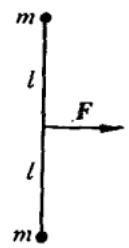
\includegraphics[width=0.1\textwidth]{figures/图3_2.jpg}
\end{center}

\vfill

\textbf{3-4} 如图所示, 表面光滑, 高 $h$、倾角 $\phi$ 的劈形物块以恒定速度 $u$ 水平朝右运动, 在其斜面顶端有一个质量 $m$ 的小木块从相对静止状态开始滑到底端.

(1) 计算小木块相对劈形物块的末速度大小 $v'$ ;

(2) 在地面系计算小木块动能总增量 $\Delta E_{k}$ ;

(3) 在地面系计算斜面支持力 $N$ 对小木块所作总功 $W_{N}$ ;

(4)在地面系验证 $W_{N} + W_{g} = \Delta E_{k}$ ，其中 $W_{g}$ 是重力对小木块所作总功.

\begin{center}
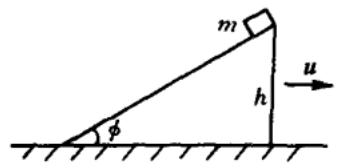
\includegraphics[width=0.25\textwidth]{figures/图3_4.jpg}
\end{center}

\vfill

\newpage

\textbf{3-5} 两个仅可压缩的轻弹簧组成的水平弹簧组如图所示, 弹簧 1 和 2 的劲度系数分别为 $k_{1}$ 和 $k_{2}$ , 它们的自由长度相差 $l$ . 建立图示的 $x$ 轴, 原点位于弹簧 2 的自由端, 图中长挡板的位置记为 $x$ . 系统势能 $E_{\mathrm{p}}(x)$ 零点按下述两种方式设定, 分别在 $0 \leqslant x \leqslant l$ 和 $x < 0$ 两个范围导出 $E_{\mathrm{p}}(x) - x$ 关系式: 

(1) 设定 $x = 0$ 点为系统势能零点; 

(2) 设定 $x = l$ 点为系统势能零点.


\begin{center}
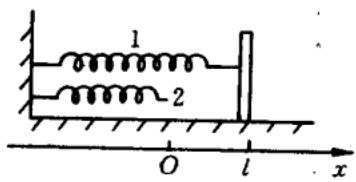
\includegraphics[width=0.25\textwidth]{figures/图3_7.jpg}
\end{center}

\vfill

\textbf{3-6} 地震的里氏(Richter)震级 $M$ 与从其释放出来的能量 $E$ 之间的关系为
\[
\log E = 5. 2 4 + 1. 4 4 M,
\]
式中 $E$ 的单位为 $J$. 1679 年 9 月 2 日, 北京地区发生过一次 8 级地震, 试求该次地震释放的能量.

长江源头为青海高原昆仑山南麓的沱沱河，从这里经 $5000\mathrm{m}$ 落差注入东海，它的水利资源的储存量按功率计为 $1.125 \times 10^{8} \mathrm{kW}$ . 试比较长江一天内所提供的水利资源能量与上述地震释放的能量哪一个大？估算长江的平均流量.

\vfill

\newpage

\textbf{3-7} 杂技演员站在蹦床上不动时,网下沉 0.20 $m$,试问当演员从 10.0 $m$ 高处自由下落时,蹦床网将受到的最大压力是杂技演员自身重力的多少倍(给出 3 位有效数字)?已知网的下沉量与正压力的二次方根成正比.


\vfill

\textbf{3-8} 如图所示, 用细绳悬挂一个匀质圆环, 环上穿两个质量相同的小串珠, 小串珠与环之间无摩擦. 令小串珠从环顶左、右两侧自静止开始自由滑下, 为使过程中环会上升, 试求环的质量与一个小串珠的质量之比 $\gamma$ 的可取值.

\begin{center}
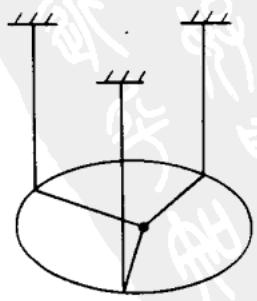
\includegraphics[width=0.2\textwidth]{figures/图3_12.jpg}
\end{center}

\vfill

\newpage

\textbf{3-9} 大质量车厢在水平地面上以 $v_{0}$ 速度匀速行使, 车厢内有一半径 $R$ 的光滑半圆柱面, 顶部有一质量为 $m$ 的小球. 开始时小球静止, 如图所示, 而后因微小扰动下滑离开圆柱面, 试求过程中圆柱面支持力 $N$ 对小球所作功.

\begin{center}
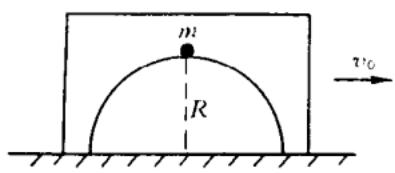
\includegraphics[width=0.25\textwidth]{figures/图3_10.jpg}
\end{center}

\vfill

\textbf{3-10} 用三根等长轻线, 将质量均匀分布的圆环对称地悬挂在天花板下, 构成一个扭摆, 小角度扭转周期为 $T_{0}$ . 再用三根轻质辐条在圆环中心固定一个与环质量相同的小物块, 如图所示, 保持扭转幅度相同, 新系统扭转周期记为 $T$ , 试求 $T$ 与 $T_{0}$ 的比值 $\gamma$ .

\begin{center}
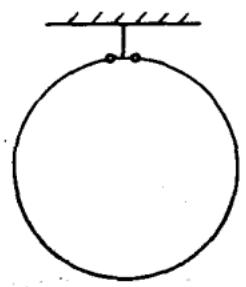
\includegraphics[width=0.2\textwidth]{figures/图3_8.jpg}
\end{center}


\vfill

\newpage

\textbf{3-11} 系统如图所示, $A$ 和 $B$ 是两个质量相同的小球, 其间是一根轻杆, 竖直线代表竖直光滑墙, 水平线代表水平光滑地面, 开始时 $\theta = 0$ , $A$, $B$ 及杆静止, 而后因微小扰动而下滑, 试问 $\theta$ 达到何值时 $A$ 球离墙?

\begin{center}
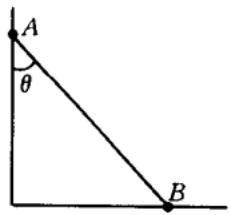
\includegraphics[width=0.2\textwidth]{figures/图3_13.jpg}
\end{center}

\vfill

\textbf{3-12} 系统如图所示, 细绳的质量线密度为常量 $\lambda$ , 长 $\pi R + H$ , 其中 $\pi R$ 段搭在半径 $R$ 且固定不可转动的滑轮上, 绳与滑轮光滑接触. 绳左侧 $H$ 段的下端恰好与水平地面自由接触, 绳的右端连接质量 $m = \frac{1}{2} \lambda H$ 的小重物. 开始时系统处于运动状态, 小重物具有竖直向下的速度 $v_0$ , 绳中各部位也具有沿绳方向的速度 $v_0$ . 为使小重物能在滑轮右侧着地, 试求 $v_0$ . (假设已有图中未画出的装置, 使绳不会甩离滑轮.)

\begin{center}
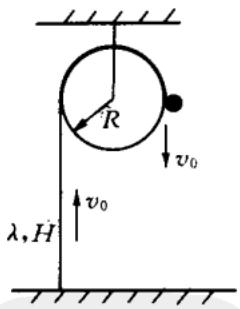
\includegraphics[width=0.2\textwidth]{figures/图3_14.jpg}
\end{center}

\vfill

\newpage

\textbf{3-13} 如图所示, 两个等高的小定滑轮相距 2 $m$, 物块 $A$ 和 $B$ 的质量各为 1 kg, 它们之间用轻绳连接, 在绳的水平段中点挂一个质量 1.9 kg 的小物块 $C$, 开始时均处于静止状态. 而后 $C$ 被释放, 三物块同时开始运动, 当 $C$ 下降 0.75 $m$ 时, 试问:

(1) $A$, $B$, $C$ 的速度各是多少?

(2) $A$, $B$, $C$ 的加速度各是多少?

\begin{center}
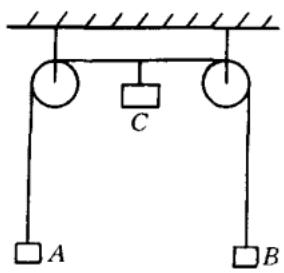
\includegraphics[width=0.2\textwidth]{figures/图3_15.jpg}
\end{center}

\vfill

\textbf{3-14} 如图所示, 两根长度同为 $l$ 的轻杆用质量 $m$ 的球形铰链相接, 两杆另一端分别连接质量 $m$ 和 $2m$ 的小球. 开始时两杆并拢竖立在光滑水平面上, 铰链球在上, 而后从静止释放, 下面两球朝两侧滑动, 两杆始终在同一竖直平面内. 略去所有阻力, 试求:

(1) 铰链球碰到桌面时的速度；

(2) 两杆夹角为 $90^{\circ}$ 时, 质量为 2m 的小球速度.

\begin{center}
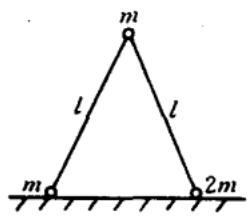
\includegraphics[width=0.2\textwidth]{figures/图3_18.jpg}
\end{center}

\vfill

\newpage

\textbf{3-15} 一个足够深, 长 $l$ 、宽 $b$ 的矩形盛水鱼缸放在车厢内, 缸的长边方向与车厢长边方向一致. 火车匀速行进时, 水面与缸口相距 $h$ . 某时刻开始, 火车作加速度为常量 $a$ 的直线运动, 为使水不溢出, 求 $a$ 的最大可取值, 设缸中水面可近似处理为始终保持平面形状.

\vfill

\textbf{3-16} 核电站的原子能反应堆中需要用低速热中子维持缓慢的链式反应, 反应释放的却是高速快中子. 反应堆中通过快中子与石墨棒内碳原子 $\left(^{12}_{6}\mathrm{C}\right)$ 的不断碰撞逐渐减速，最后成为所需要的热中子。将快中子与热中子的平均动能分别设为 $2.0\times10^{6}eV$ 和 $0.025eV$ ，每次碰撞前碳原子均处于静止状态，碰撞为弹性。试问经过多少次碰撞，快中子可成为热中子？


\vfill

\newpage

\textbf{3-17} “弹弓效应”是航天技术中增大宇宙探测器速率的一种有效方法. 如图所示, 土星以相对于太阳的轨道速率 $v_{M}=9.6$ km/s 运行, 一空间探测器以相对于太阳的速率 $v_{0}=10.4$ km/s 迎向土星飞行. 由于土星的引力, 探测器绕过土星沿着和原来相反的方向离去,试求探测器离去时相对于太阳的速率 $v$.

\begin{center}
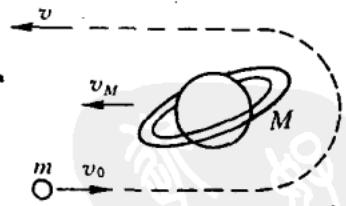
\includegraphics[width=0.25\textwidth]{figures/图3_21.jpg}
\end{center}

\vfill

\textbf{3-18} 如图所示，滑块 $A_{1}$ 和 $A_{2}$ 由轻杆连接成一个整体，其质量为 $M$，轻杆长 $L$，滑块 $B$ 的质量为 $m$，长为 L/2，其左端有一小槽, 槽内装有轻质弹簧. 开始时 $B$ 紧贴 $A_{1}$ , 弹簧处于压缩状态, 今突然松开弹簧, 整个系统获得动能 $E_{\mathrm{k}}$ . 弹簧松开后不再起任何作用, 以后 $B$ 将在 $A_{1}, A_{2}$ 之间发生弹性碰撞. 假定整个系统都放在光滑水平面上, 试求物块 $B$ 的运动周期 $T$ .

\begin{center}
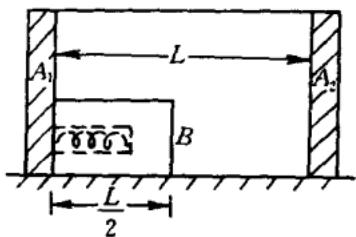
\includegraphics[width=0.25\textwidth]{figures/图3_22.jpg}
\end{center}

\vfill

\newpage

\textbf{3-19} 在水平冰面上兄弟俩作推车游戏, 哥哥质量 $m_{1}$ , 弟弟质量 $m_{2}$ , 小车质量 $m$ . 开始时哥哥与小车静止在同一地点, 弟弟静止在另一地点. 而后, 哥哥将小车朝着弟弟推去, 小车推出后相对于哥哥的速度大小为 $u$ . 弟弟接到小车后又将小车推向哥哥, 小车推出后相对于弟弟的速度大小仍为 $u$ . 哥哥接到小车后又再次将小车推向弟弟, 如此继续下去. 设冰面光滑, 且足够大.

(1) 若某次弟弟推出的小车恰好追不上哥哥, 试求三者各自的运动速度大小;

(2) 若无论 $u$ 取什么样的非零值, 弟弟第一次推出的小车都是恰好追不上哥哥，试给出 $m_{1}, m_{2}, m$ 之间需满足的关系式.

\vfill

\textbf{3-20} 质量 $m$ 的均匀圆环形光滑细管道放在光滑水平大桌面


上，管内有两个质量同为 $m$ 的小球 $A$ 和 $B$ 位于一条直径的两端. 开始时管道静止， $A$ 和 $B$ 沿着切线方向有相同速度 $v_0$ ，如图所示． $A, B$ 间碰撞的恢复系数 $e = \frac{\sqrt{3}}{3}$ ，试求：

(1) $A$, $B$ 第一次碰撞前瞬间的相对速度大小 $u$;

(2) $A$, $B$ 第二次碰撞前瞬间各自相对大桌面的速度大小 $v'$ .

\begin{center}
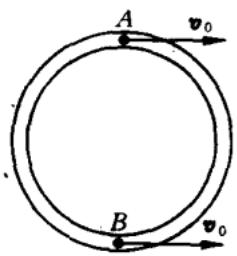
\includegraphics[width=0.2\textwidth]{figures/图3_24.jpg}
\end{center}

\vfill

\newpage

\textbf{3-21} 小球 $A, B$ 在光滑水平面上沿同一直线朝着对方运动， $A$ 球质量大于 $B$ 球质量。已知碰前两球动能相同，碰后 $A$ 球速度为零， $B$ 球速度不为零，试求 $A$ 球质量与 $B$ 球质量之比 $\gamma$ 。

\vfill

\textbf{3-22} 长平板在水平方向上以恒定的速度 $v_{0}$ 朝右运动，板上方 $H$ 高处有一小球自静止自由下落与平板碰撞。已知球与平板间摩擦因数 $\mu=0.1$ ，小球反弹高度仍为 $H$，试确定图 3-25 中小球反弹抛射角 $\phi$ 的正切 $\tan\phi$ 与 $\sqrt{H}$ 之间的函数关系。

\begin{center}
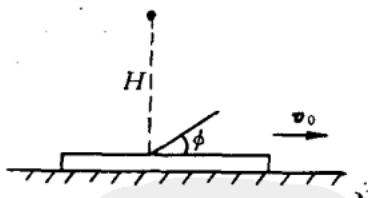
\includegraphics[width=0.3\textwidth]{figures/图3_25.jpg}
\end{center}

\vfill

\newpage

\textbf{3-23} 一斜面体静放在光滑水平地面上, 斜面倾角 $\theta = 15^{\circ}$ . 如图所示, 小球从静止自由下落到光滑斜面, 下落高度 $h = 1.60 \mathrm{~m}$ , 碰撞点距地面高度 $H = 1.00 \mathrm{~m}$ . 小球与斜面法向碰撞恢复系数 $e = 0.60$ , 碰后斜面体不离地, 小球与斜面体的质量比 $m / M = 0.5$ .

(1) 求碰后小球反弹速度和斜面体获得的速度；

(2) 求碰后小球最高位置相对原碰撞点的高度；

(3) 判断小球碰后将落于斜面还是落于地面?

\begin{center}
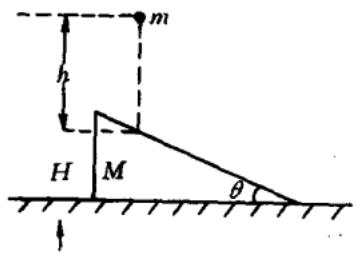
\includegraphics[width=0.25\textwidth]{figures/图3_26.jpg}
\end{center}

\vfill

\textbf{3-24} 三个编号分别为 1,2,3 的相同匀质光滑小立方块，按图 3-28 所示方式放在光滑水平面上，直径与立方块边长相同的匀质光滑小圆柱块沿着图中对称方向以速度 $u_0$ 运动过来，接着便发生弹性碰撞。已知圆柱块质量是每一立方块质量的 2 倍，试求碰后各物块运动速度大小 $v_1, v_2, v_3$ 和 $u$ 。

\begin{center}
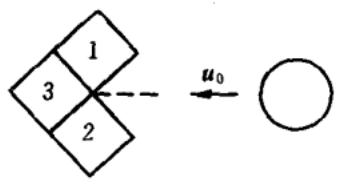
\includegraphics[width=0.25\textwidth]{figures/图_3_28.jpg}
\end{center}

\vfill

\newpage

\textbf{3-25} 在一水平面上有两根相互平行的固定导轨 $M_{1}N_{1}$ 和 $M_{2}N_{2}$ , 质量 $m_{1}$ 的物块 $P_{1}$ 穿在 $M_{1}N_{1}$ 上, 质量 $m_{2}$ 的物块 $P_{2}$ 穿在 $M_{2}N_{2}$ 上, $P_{1}$ 与 $P_{2}$ 间用一根不可伸长的轻绳连接, 开始时绳处于松弛状态. 今使 $P_{1}$ 获得沿导轨方向速度 $v_{0}, P_{2}$ 静止, 如图所示. 设系统处处无摩擦, $P_{1}$ 运动一段时间后绳被拉直,其内产生拉力,同时使导轨与相应的物块间有力的作用,这些力的作用时间 $\Delta t$ 非常短.试就下述两种情况,计算 $\Delta t$ 刚结束时 $P_{1}$ 和 $P_{2}$ 运动速度 $u_{1}$ 和 $u_{2}$ .

(1) 绳的作用不损耗系统动能；

(2) 绳的作用使 $P_{1}$ 和 $P_{2}$ 沿绳长方向的速度相同.

\begin{center}
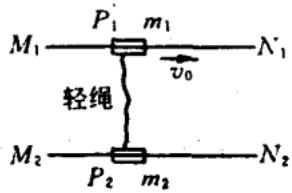
\includegraphics[width=0.2\textwidth]{figures/图3_30.jpg}
\end{center}

\vfill

\section*{B 组}
\vspace{0.3cm}
\textbf{3-26} 一架质量 $M = 810\mathrm{kg}$ 的直升飞机，靠螺旋桨的转动使 $S = 30\mathrm{m}^2$ 面积内的空气以 $v_{0}$ 速度向下运动，从而使飞机悬停在空中. 已知空气密度 $\rho_0 = 1.20\mathrm{kg / m^3}$ ，求 $v_{0}$ 大小，并计算发动机的最小功率 $p$ .


\vfill

\newpage

\textbf{3-27} 内外半径几乎同为 $R$ 的竖直固定圆环管，底部有一质量为 $m$ 的小球，环内有根轻绳连接小球，绳的另一端从管的上方缺口水平引出，绳与管壁间摩擦可略。用力 $F$ 将绳拉出，并保证小球在运动的过程中始终具有原始的速率 $v_{0}$ 。设圆环管的外壁、内壁与小球的摩擦因数分别为 $\mu_{1}, \mu_{2}$ ，试求小球从图3-31所示位置到达最高位置的过程中，力 $F$ 所作功 $W$ 。

\begin{center}
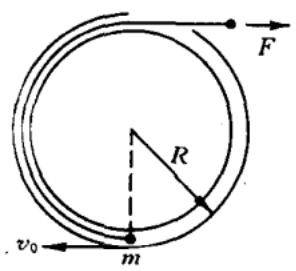
\includegraphics[width=0.2\textwidth]{figures/图3_31.jpg}
\end{center}

\vfill

\textbf{3-28} 在航天飞船上,如图所示,有一个长 $l=20\ cm$ 的圆筒绕着与筒的长度方向垂直的轴 MN 以恒定的角速度$\omega = \frac{10}{3}\pi \mathrm{s}^{-1}$ 旋转. 筒的近轴端与轴相距 $d = 10\mathrm{cm}$ , 筒内装满非常黏稠、密度 $\rho = 1.2\mathrm{g/cm^3}$ 的液体. 有一个质量 $m' = 1.0\mathrm{mg}$ 、密度 $\rho' = 1.5\mathrm{g/cm^3}$ 的颗粒 $P$ , 从圆筒中央位置静止释放, 试求 $P$ 在到达筒端过程中克服液体黏性阻力所作功. 又问, 如果 $P$ 的密度 $\rho'' = 1.0\mathrm{g/cm^3}$ , 其他条件不变, 则 $P$ 在到达筒端过程中克服液体黏性阻力所作功又是多少?

\begin{center}
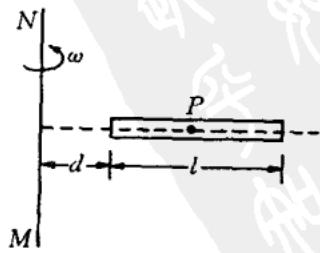
\includegraphics[width=0.2\textwidth]{figures/图3_33.jpg}
\end{center}

\vfill

\newpage

\textbf{3-29} 两个核子之间的相互作用势能可表述为 $U(r) = -\frac{r_0}{r} U_0 \mathrm{e}^{-r / r_0}$ , 这便是汤川(Yukawa)势. 式中 $r_0 (r_0 = 1.5 \times 10^{-15} \mathrm{~m})$ , $U_0 (U_0 = 50 \mathrm{MeV})$ 均为常量.

(1) 给出两个核子之间相互作用力的表达式；

(2) 计算当 $r=2r_{0},5r_{0},10r_{0}$ 时的作用力与 $r=r_{0}$ 时的作用力之比, 由此可见此种力的短程特征.


\vfill

\textbf{3-30} 地面上有一固定的点电荷 $A$. $A$ 的正上方有另一带电质点 $B$，在重力和库仑斥力作用下，$B$ 在 $A$ 的正上方 $H$ 到 H/2 高度间往返运动，试求 $B$ 的最大运动速度 $v_{max}$ .


\vfill

\newpage

\textbf{3-31} 将劲度系数为 $k$ 、自由长度为 $L$ 、质量为 $m$ 的均匀柱形弹性体竖直朝下，上端固定，下端自由. 开始时弹性体处处无形变，而后在重力作用下各部位发生运动和形变,因为空气阻力等作用,最后弹性体处于静止状态,试求弹性体的弹性势能和重力势能的各自增量.


\vfill

\textbf{3-32} 各边长为 $l$ 的匀质立方体大木块, 如图所示, 对半切成两块, 将上表面为 $AB_{1}CB_{2}$ 斜平面的一块留下放在水平面上, 其质量为 $2m$ . 沿 $AB_{1}, AB_{2}, B_{1}C, B_{2}C$ 设置四根斜直细管道, 质量均为 $m$ 的两个小球同时从 $A$ 端静止释放, 分别沿 $AB_{1}C, AB_{2}C$ 管道滑下, 它们在 $B_{1}, B_{2}$ 处可光滑迅速地拐弯.

(1) 设木块固定在水平面上，管道平直部分与各小球之间的摩擦因数同为 $\mu$ ，试问 $\mu$ 为何值，小球才能滑下？并计算小球到达 $C$ 处时的速度.

(2) 设木块与水平面光滑接触, 管道内处处无摩擦, 试求小球到达 $C$ 处时相对地面的速度大小.


\begin{center}
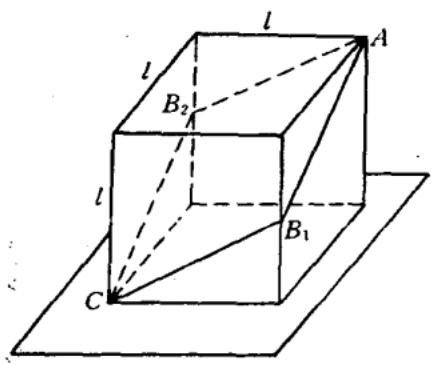
\includegraphics[width=0.2\textwidth]{figures/图3_35.jpg}
\end{center}

\vfill

\newpage

\textbf{3-33} 如图所示, 质量 $2m$ 的小环套在水平光滑的固定细杆上, 并用长 $l$ 的轻线与质量为 $m$ 的小球相连. 今将轻线沿水平拉直, 使小球从与环等高处由静止释放, 试问当轻线与水平杆夹角为 $\theta$ 时线中张力 $T$ 为多大?

\begin{center}
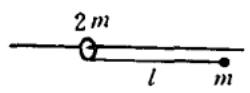
\includegraphics[width=0.2\textwidth]{figures/图3_37.jpg}
\end{center}

\vfill

\textbf{3-34} 在一个带有活塞的固定柱形汽缸内有一单原子分子沿着汽缸的长度方向往返运动,它与汽缸左壁及活塞均作弹性正碰撞.


(1) 如图所示, 设汽缸的初始长度为 $l_{0}$ , 活塞推进速度为常量 $u$ , 分子从活塞近旁以 $v_{0} \gg u$ 的初始速率朝汽缸左壁运动. 略去重力影响, 试确定分子与活塞多次碰撞后, 其速率 $v$ 与汽缸长度 $l$ 之间的关系.

(2) 设汽缸截面积为 $S$，则汽缸初始体积 $V_{0}=S \cdot l_{0}$ ，汽缸长度为 $l$ 时的体积 $V=S \cdot l$ 。再为该分子引入“温度”量 $T$，使其正比于分子的动能，试求 $T$ 与 $V$ 之间的关系。

\begin{center}
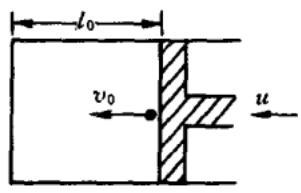
\includegraphics[width=0.25\textwidth]{figures/图3_39.jpg}
\end{center}

\vfill

\newpage

\textbf{3-35} 光滑水平桌面上静止放置若干个相同的匀质光滑小球，打击其中某个球，与别的球逐个弹性碰撞经一闭合路线后又可停在原位置上，试问至少需放多少个球？给出一种球的放置图.


\vfill

\textbf{3-36} 小球从水平地面上以初速 $v_{0}$ 斜抛出去, 小球落地时在竖直方向上发生的非弹性碰撞恢复系数为 $e$, 小球与地面间的摩擦因数为 $\mu$ . 若要求小球第一次与地面碰撞后能竖直弹起, 试求小球可能达到的最大水平射程 $s_{max}$ .


\vfill

\newpage

\textbf{3-37} 如图所示, 质量 $M$、倾角 $\phi$ 的斜面体静放在光滑水平面上, 质量 $m$ 的小球以水平速度 $v_{0}$ 与斜面发生碰撞, 设小球与斜面间无摩擦, 且碰撞无动能损失.

(1) 试求碰后小球沿斜面方向的速度 $v_{\parallel}$ 和垂直于斜面方向速度 $v_{\perp}$ ，以及斜面体沿地面运动速度 $u$；

(2) $M, m, \phi$ 之间满足什么样的关系，能使小球碰后速度竖直向上？

\begin{center}
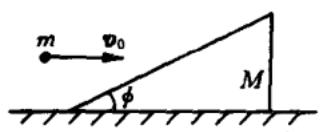
\includegraphics[width=0.2\textwidth]{figures/图3_43.jpg}
\end{center}

\vfill

\textbf{3-38} 质量相同的两个小球 $A$ 和 $B$ 用长 $L$ 轻绳连接, 开始时都静止在光滑的水平桌面边缘. 今使 $B$ 球以 $v_{0} = \sqrt{\frac{gL}{2\sqrt{2}}}$ 的初速水平抛出, 如图所示. 设绳不损耗机械能, 试求绳伸直后很短时间内因绳的作用而使 $A, B$ 各自具有的速度 $\pmb{v}_{A}, \pmb{v}_{B}$ .

\begin{center}
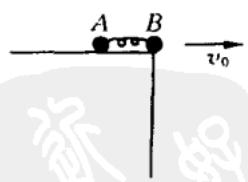
\includegraphics[width=0.2\textwidth]{figures/图3_46.jpg}
\end{center}


\vfill

\newpage
